% Phase 3 (CP3a-CP3d). Each subsection is a separate file so checkpoints stay independent.
% Order set by D17 (2026-09-19): modeling before control, matching the claim ledger and the
% narrative arc. The headline number therefore lands in 03c, not 03b.
\section{Experiments}
\label{sec:exp}
% RQ lead added 2026-09-20. Two top-level questions, one per experiment line, each with named
% sub-questions so that the subsection conclusions can answer them by label. Mapping to the
% Introduction: contribution 1 <-> RQ1a, contribution 2 <-> RQ1b, contribution 3 <-> RQ2.
The experiments answer two questions, one per experiment line.
\textbf{RQ1 (modeling).} Does the learned operator predict a multi-turn attribute from observable readings alone?
It splits into three parts: (1a) whether history beyond the current turn improves prediction over the current reading alone (\S\ref{sec:exp_prediction}); (1b) whether the linear special case reported as ours is matched or beaten by a learned nonlinear lifting or by a recurrent sequence model (\S\ref{sec:exp_prediction}); and (1c) what the memory state carries, how many past readings it needs and whether its gain is inter-turn dynamics or a fixed level per prompt item (\S\ref{sec:exp_memory}).
\textbf{RQ2 (control).} Does predictive control built on that operator raise constraint satisfaction on a frozen model?
It splits into two parts: (2a) against the same model with no control, and (2b) against two white-box latent controllers that read the model's activations, where ours reads only text (\S\ref{sec:exp_control}).
\S\ref{sec:exp_analysis} is an analysis rather than a further question: it states the conditions under which a gain on RQ1 can become a gain on RQ2.
\subsection{Experimental Setup}
\label{sec:exp_setup}

Experiments cover two task groups.
The first is self-built multi-turn tasks that form the modeling line.  % RECOVERED 2026-09-19 (Opus); semantic.md Experiments P1
Table~\ref{tab:prediction} carries seven of them: sentence length, items (s2), items (s1), sentiment, defense, constraint and CEFR.  % tab_prediction.tex column headers, updated 2026-09-19
Appendix~\ref{app:A2_small_columns} separately reports sentiment, average word length, defense and GSM8K-sharded for completeness.  % _build_report.json:prediction_appendix
Character length and formality are not shown in either table this round.  % table1_swap_2026-09-19
The second group is three public instruction-following benchmarks that form the control line: IFBench, IFEval and COLLIE.  % contract.yaml meta.benchmarks
Together they carry eleven subtasks: WC, UWC, NS and NP for IFBench; KF, WC, NS and NP for IFEval; Word, Sent. and Para. for COLLIE.  % contract.yaml meta.benchmarks
The modeling line runs on a single model, Qwen3-4B-Instruct-2507, which both produces and scores the self-built trajectories.  % RECOVERED 2026-09-19 (Opus, docs/LEDGER.md lines 201-202, 549)
A second backbone for the modeling line remains a planned arm with no submitted job, so every number in Table~\ref{tab:prediction} comes from that one model.  % RECOVERED 2026-09-19 (Opus, docs/NAMING.md backbone2 row)
The control line is separate: it reports two frozen target models, Qwen3-4B and Qwen3-8B, on runs supplied by a co-author.  % tab_control.tex row groups; c5 notes

The modeling line compares six predictors, the six rows of Table~\ref{tab:prediction}.  % tab_prediction.tex row count
Stateless is a memoryless null, Last-turn is a single-reading state, and Memory w/o action is a multi-turn state without the command term.
LSTM is a recurrent sequence baseline, and KOMPAS (learned lifting) and KOMPAS (linear) are the two operator variants.
KOMPAS (linear) sets the encoder and decoder to the identity map of \S\ref{sec:model}, the reported instance throughout this paper.
Window length and horizon vary by task: window length ranges from 1 to 4 readings and horizon from 3 to 6 steps, with full per-task settings in Appendix~\ref{app:A3_window}.  % RECOVERED 2026-09-19 (Opus, tabulated from evidence/numbers.yaml); semantic.md Experiments P2
Scored held-out rows per task range from 30 to 12,376, counted after windowing.  % RECOVERED 2026-09-19 (Opus, evidence/numbers.yaml)
The trajectories those rows come from number 40 to 100 for the seven columns of Table~\ref{tab:prediction}, and 4 to 30 for the appendix columns.  % RECOVERED 2026-09-19 (Opus, group counts in evidence/numbers.yaml `test` fields)
Every interval reported in \S\ref{sec:exp_prediction} is a paired grouped bootstrap over trajectories, with 2000 resamples.  % evidence/numbers.yaml `test` field, all n_main_* contrast rows

The control line compares four methods per frozen model, the four rows of Table~\ref{tab:control}: Base, TMPC, RE-Control and KOMPAS.  % tab_control.tex row count
Base applies no control, and its Access entry is `--' in Table~\ref{tab:control}.  % tab_control.tex Access column
TMPC and RE-Control are white-box latent controllers that require activation access to the frozen model.  % tab_control.tex Access column
KOMPAS needs only the instruction it sends, marked black-box Access, since it never opens the model.  % tab_control.tex Access column
% CITE: wang2026tmpc
% CITE: kong2024recontrol
TMPC and RE-Control are reproductions by a co-author rather than baselines the authors ran themselves.  % c6 notes

A predictor that never beats guessing the best fixed trivial answer scores zero, and one that halves that guess's error scores one half.
We define the prediction skill score as
\begin{equation}
    \mathrm{Skill}_H
    =
    1-\frac{\sum_{h=1}^{H}\ell_h}{\sum_{h=1}^{H}\ell_h^{\mathrm{null}}},
    \label{eq:skill}
\end{equation}
Here $\ell_h$ is the squared forecast error at horizon step $h$, defined in Section~\ref{sec:problem_modeling}.  % contract.yaml symbol_lattice s_ell
The numerator sums it over the horizon, and $\ell_h^{\mathrm{null}}$ is the same quantity for the best trivial null.  % contract.yaml symbol_lattice s_ellnull
The best trivial null is the best-scoring memoryless baseline over the same rows.
The score $\mathrm{Skill}_H$ is therefore the fraction of that null's horizon error which the operator removes.  % contract.yaml symbol_lattice s_skill
A score of zero means tied with that null; a negative score means worse than it.

The control-line metric is the constraint-satisfaction score as reported for each benchmark, a per-subtask percentage with no interval attached.  % numbers_benchmark.yaml unit field
% TODO(data): metric definition pending from colleague
Its exact definition, what counts as a satisfied instruction per subtask, is not yet available from the colleague.
The two experiment lines therefore report different metrics in different reference frames.
The modeling line's skill score is referenced against a best-trivial-null baseline and can go negative, while the control line's percentage carries no reference point.
The modeling line tests whether the operator predicts the trajectory; the control line tests whether acting on that prediction changes the outcome.

% Phase 3 CP3b. Modeling line: does the learned operator predict? Table 1 = tables/tab_prediction.tex.
\subsection{Predictive Accuracy of the Learned Operator}
\label{sec:exp_prediction}

\textbf{Question.} RQ1a and RQ1b: whether multi-turn history improves prediction over the current reading alone, and whether a learned nonlinear lifting or a recurrent sequence model beats the linear special case reported as ours.
\textbf{Setup.} Setup, tasks and baselines follow \S\ref{sec:exp_setup}; Table~\ref{tab:prediction} reports the skill score defined there.

% GENERATED by tools/build_tables.py. Do not edit by hand; edit the evidence ledger instead.
% MAIN-TEXT TABLE 1 of 2 (modeling line). D18: the main text carries exactly two tables.
\begin{table}[t]
\centering
\caption{Free-running prediction skill on seven multi-turn tasks. Higher is better. Best per column in bold, second underlined.}
\label{tab:prediction}
\footnotesize
\resizebox{\textwidth}{!}{
\begin{tabular}{lccccccc}
\toprule
Predictor & Sentence len. & Items (s2) & Items (s1) & Char. len. & Formality & Constraint & CEFR \\
\midrule
Stateless & 0.000 & 0.000 & 0.000 & 0.000 & 0.000 & 0.000 & 0.000 \\  % n_main_002 n_main_034 n_main_018 n_main_066 n_main_082 n_main_121 n_main_169
Last-turn & 0.166 & 0.514 & 0.395 & 0.034 & \textbf{0.414} & 0.285 & 0.518 \\  % n_main_006 n_main_038 n_main_022 n_main_070 n_main_086 n_main_123 n_main_171
Memory w/o action & \underline{0.764} & \underline{0.824} & 0.615 & \underline{0.291} & 0.357 & 0.517 & \underline{0.561} \\  % n_main_008 n_main_040 n_main_024 n_main_072 n_main_088 n_main_125 n_main_173
LSTM & 0.750 & 0.808 & \underline{0.634} & \textbf{0.301} & 0.373 & \textbf{0.546} & -0.101 \\  % n_main_012 n_main_044 n_main_028 n_main_076 n_main_092 n_main_127 n_main_175
KOMPAS (learned lifting) & 0.752 & 0.821 & 0.627 & 0.239 & \underline{0.385} & 0.471 & -0.032 \\  % n_main_010 n_main_042 n_main_026 n_main_074 n_main_090 n_main_129 n_main_177
KOMPAS (linear) & \textbf{0.769} & \textbf{0.826} & \textbf{0.640} & 0.269 & 0.379 & \underline{0.519} & \textbf{0.567} \\  % n_main_004 n_main_036 n_main_020 n_main_068 n_main_084 n_main_131 n_main_179
\bottomrule
\end{tabular}
}
\end{table}


\textbf{Findings, ranking and history.} The linear special case, KOMPAS (linear), ranks first on four of seven columns: sentence length, Joint-3, Joint-2 and CEFR.  % c4; ours_best_of_7=4 (n_main_004 n_main_036 n_main_020 n_main_179)
It ranks second on the remaining three: sentiment, defense and constraint.
The driver is that all three second places are close: the linear case trails the top method by no more than 0.034 in point-estimate skill score.  % c4 driver_keyword  % ours_second_of_7=3 (n_main_100 sentiment; n_main_147 defense; n_main_131 constraint)
History beyond the current turn beats the current reading on four of seven columns, with paired bootstrap intervals excluding zero.  % c1; contrasts.ours_minus_last_turn (n_main_013 n_main_045 n_main_029 n_main_109 n_main_148 n_main_132 n_main_180)
The three exceptions are Joint-2 and sentiment, whose intervals contain zero, and defense, whose point estimate is negative with an interval containing zero.  % n_main_029 Joint-2 (vector_count_stage1); n_main_109 sentiment; n_main_148 defense
The driver is that the window exposes both level and trend, which a single reading cannot carry.  % m1

\textbf{Findings, lifting and LSTM.} A learned nonlinear lifting never beats the identity lifting with an interval excluding zero, on any of the seven columns.  % c2; contrasts.ours_minus_nonlinear
It loses on three of them, with the largest gap on CEFR at +0.599 in favor of the linear case.  % contrasts.ours_minus_nonlinear:tsar_cefr=0.599 (n_main_183)
The driver is that the attribute readouts are low-dimensional, one scalar per attribute and at most three per task, leaving a learned lifting little structure to expose.  % m4; Joint-2/Joint-3 are 2- and 3-dimensional, the rest scalar
Against an LSTM sequence baseline, comparisons split three ways with intervals excluding zero: two favor the linear case, one favors the LSTM.  % c3; contrasts.ours_minus_lstm
Joint-3 and CEFR favor the linear case, while constraint favors the LSTM.  % n_main_048 n_main_182 favor linear; n_main_134 favor LSTM
No mechanism is established for the LSTM win, and none is proposed here.  % c3 driver_keyword: no mechanism established

Together, \uline{history beyond the current turn beats the current reading on four of seven tracked attributes, which answers RQ1a yes on those four. Neither a learned lifting nor an LSTM sequence model beats the reported linear special case on balance, which answers RQ1b no.}

% Side experiments P1 (memory depth) and P2 (item intercept), added 2026-09-19.
% Plan: claude/side_experiments_plan_2026-09-19.md. Results archive: docs/experiments/paper_side_experiments_results.md.
% The figure is generated by tools/build_figs.py from evidence/numbers.yaml; the ids behind every mark are in figs/_fig_report.json.
% 2026-09-20: the former Figures 2 and 3 were merged into one three-panel figure, and the
% reading rules that stood in their captions moved into the Setup and Findings text.
\subsection{What the Memory State Carries}
\label{sec:exp_memory}

\textbf{Question.} RQ1c, in two parts: how many past readings the state needs, and whether the gain from memory is inter-turn dynamics or a fixed level per prompt item.
\textbf{Setup.} Tasks, baselines and the skill score follow \S\ref{sec:exp_setup}; both experiments vary one thing in the KOMPAS (linear) row of Table~\ref{tab:prediction}.
Table~\ref{tab:prediction} fits each row on every transition its state can be formed from, so a one-reading state trains on earlier turns than a four-reading state.  % paper_side_experiments_results.md section 1.2, default caliber
Both experiments here fit every depth on the same set of transitions, which separates the depth of the state from the size of its training set.  % matched caliber; figs/_fig_report.json
Under that matched window the memory gain on sentence length shrinks from +0.603 in Table~\ref{tab:prediction} to +0.109, so the two calibers answer different questions.  % n_main_013 (default) vs n_abl_127 (matched)
In every panel of Figure~\ref{fig:memory} a filled marker means the 95\% paired bootstrap interval excludes zero, and a hollow marker means it contains zero.  % moved out of the former Figure 2 and Figure 3 captions, 2026-09-20

\begin{figure}[t]
\centering
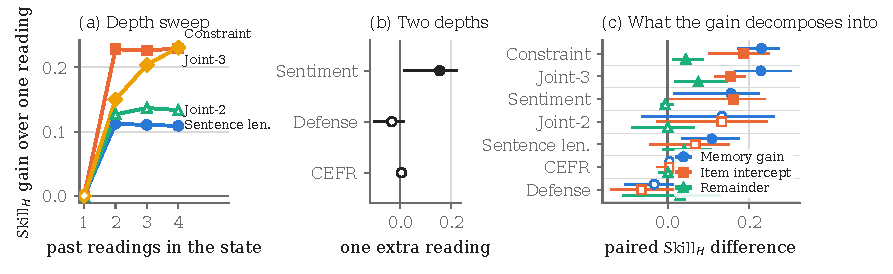
\includegraphics[width=\linewidth]{figs/fig_memory.pdf}
\caption{How deep the memory state has to be, and what its gain decomposes into, both under a matched training window. (a) Gain of a state holding $d$ past readings over a state holding one, on the four tasks whose design allows a sweep. (b) The same gain for one extra reading on the three designs that carry two depths. (c) Three paired differences per task of Table~\ref{tab:prediction}.}
\label{fig:memory}
\end{figure}

\textbf{Findings, depth.} On three of the four sweepable tasks the second reading buys the whole gain: +0.112 on sentence length, +0.228 on Joint-3, +0.127 on Joint-2.  % c10; n_abl_124 n_abl_184 n_abl_157
The third and fourth readings add no more than 0.010 on those three tasks.  % n_abl_126 n_abl_128 n_abl_186 n_abl_188 n_abl_159 n_abl_161
The Joint-2 interval contains zero at every depth.  % n_abl_157 n_abl_158 n_abl_160
Constraint is the exception: each added turn keeps paying, +0.149, +0.054 and +0.027 for the second, third and fourth, each with an interval excluding zero.  % n_abl_235 n_abl_237 n_abl_239
Of the three two-depth tasks, sentiment gains +0.155 from one extra reading, while defense and CEFR do not separate from zero.  % n_abl_151 (caveated: two cells) n_abl_245 n_abl_262
The driver is that a level and a trend take two readings to express, and the attribute tasks carry little structure beyond that pair.  % m1
No mechanism is established for why constraint keeps gaining, and none is proposed here.  % c10 notes

\textbf{Findings, item intercept.} Panel (c) carries three paired differences per task: the memory gain over Last-turn, the part an added per-item intercept recovers, and what remains beyond that intercept.  % moved out of the former Figure 3 caption
Intercepts are estimated on turns outside the scored window.  % moved out of the former Figure 3 caption
A per-item intercept added to the one-reading state recovers most of the memory gain: 81\% on constraint and 67\% on Joint-3.  % c11; n_mech_061/n_mech_060=0.807, n_mech_058/n_mech_057=0.673
What remains after the intercept is +0.045 on constraint and +0.075 on Joint-3, both with intervals excluding zero.  % n_mech_059 n_mech_056
On the other five tasks the remainder does not separate from zero, and on sentiment and Joint-2 the intercept accounts for the whole gain.  % n_mech_050 n_mech_053 n_mech_047 n_mech_068 n_mech_062; n_mech_052 vs n_mech_051, n_mech_055 vs n_mech_054
The driver is that each prompt item holds its own level across turns, and several past readings estimate that level where one reading cannot.  % m6
Inter-turn dynamics beyond that level is measured on two tasks, and it is the smaller of the two parts on both.  % c11 notes

Together, \uline{one extra reading carries most of what memory buys, and most of that is a per-item level rather than inter-turn dynamics; this answers RQ1c. A remainder attributable to dynamics is measured on two of seven tasks.}

% Phase 3 CP3c. Control line: does predictive selection raise satisfaction? Table 2 = tables/tab_control.tex.
\subsection{Constraint Satisfaction under Predictive Control}
\label{sec:exp_control}

For RQ2a and RQ2b, we ask whether predictive control using the learned operator improves constraint satisfaction over the same frozen model without control, and how it compares with two white-box latent controllers. The setup, benchmarks, and baselines are described in \S\ref{sec:exp_setup}; Table~\ref{tab:control} reports the constraint-satisfaction score defined there.

Averaged across the eleven subtasks, predictive control improves constraint satisfaction over the uncontrolled baseline by 14.5 points on Qwen3-4B and 14.8 points on Qwen3-8B. These are point estimates, with no seeds or intervals. The controller scores each candidate by its predicted trajectory rather than its immediate effect, allowing it to choose a command different from the target while the attribute is still changing.
Predictive control also outperforms the stronger white-box baseline, RE-Control, by 5.3 points on Qwen3-4B and 5.7 points on Qwen3-8B. These are also point estimates without intervals. RE-Control uses model activations, whereas predictive control operates from text alone.

Across the 22 model-by-subtask comparisons, predictive control scores higher than the uncontrolled baseline in every case and higher than both white-box controllers in every case. This count answers RQ2a and RQ2b affirmatively; it is not a claim of statistical significance.


% Phase 3 CP3d. Bridge from prediction quality to control quality, plus inference cost.
% Compressed 2026-09-21 (page budget, item A2): "the bound" and "the cost argument" merged into one
% Findings paragraph; the command-channel scope moved to Appendix A7 with a two-sentence pointer here.
\subsection{From Prediction Quality to Control Quality}
\label{sec:exp_analysis}

\textbf{Question.} Not a further RQ but the link between RQ1 and RQ2: how prediction quality relates to control quality, and where on the self-built tasks that link does not carry.
\textbf{Setup.} Setup follows \S\ref{sec:exp_setup}; the derivation is the selection bound of \S\ref{sec:prediction_control_bound}, not repeated here.

\textbf{Findings, bound and cost.} The selection bound of \S\ref{sec:prediction_control_bound} keeps the cost of the selected command within twice the estimation error of the best candidate.  % c9
It is theoretical, not measured, and it covers one held-command comparison at a single step rather than the replanned closed loop.  % c9 strength_basis: theoretical; c9 notes
Evaluating a candidate costs one linear propagation and a readout through the closed-form rollout of \S\ref{sec:control_method}, adding no query to the target model.  % c8
The driver is that the affine transition and the scalar command column collapse an $h$-step lookahead into a matrix power.  % m2

\textbf{Cross-check, the equal-cost boundary.} On the four self-built behavioral tasks, the closed loop ties the best equal-cost fixed schedule, with per-task numbers in Appendix~\ref{app:A4_equal_cost}.  % nc_2
On those four tasks the instruction's effect depends little on when it is issued, which leaves planning almost nothing to exploit.  % nc_2

\textbf{Cross-check, the command-channel scope.} On four of the seven modeling columns the applied command is an exact affine function of the memory state, so the prediction design cannot estimate an independent action effect there.  % m5; nc_1; nc_8; n_main_014 n_main_046 n_main_030 n_main_110
Appendix~\ref{app:A7_command_channel} reports the three columns where it can, all with intervals containing zero; this is a property of how the trajectories were collected, not a result about the controller.  % n_main_149 n_main_133 n_main_181; m5 notes

Combined, \uline{the selection bound links prediction error to the quality of the command selected at a single step, while candidate evaluation adds no target-model queries. The equal-cost and command-channel cross-checks delimit the conditions under which the predictive gains studied in RQ1 can translate into the control gains studied in RQ2.}

